%%%%%%%%%%%%%%%%%%%%%%%%%%%%%%%%%%%%%%%%%%%%%%%%%%%%%%%%%%%%%%%%
%
%  Template for creating scribe notes for MLPM2013.
%
%  Fill in your name, lecture number, lecture date and body
%  of scribe notes as indicated below.
%
%%%%%%%%%%%%%%%%%%%%%%%%%%%%%%%%%%%%%%%%%%%%%%%%%%%%%%%%%%%%%%%%


\documentclass[11pt]{article}

\setlength{\topmargin}{0pt}
\setlength{\textheight}{9in}
\setlength{\headheight}{0pt}
\setlength{\headsep}{0pt}
\setlength{\oddsidemargin}{0.25in}
\setlength{\textwidth}{6in}
\pagestyle{plain}

\usepackage{algorithm2e}
\usepackage{tikz}
\usetikzlibrary{arrows}
\usetikzlibrary{positioning}
\usetikzlibrary{shapes,shapes.geometric,arrows,fit,calc,positioning,automata,}
\usetikzlibrary{fit,positioning}
\usepackage{amsmath}
\begin{document}

\thispagestyle{empty}

\vspace{-0.7in}

\begin{center}
\bf\large Machine Learning Principles and Methods
\end{center}

\noindent
Lecturer:  Joris Mooij  %%% FILL IN LECTURER (if not RS)
\hfill
Lecture \#12               %%% FILL IN LECTURE NUMBER HERE
\\
Scribe: Nikolaas Steenbergen \&Efstathios Charitos \& Jerome Cremers                %%% FILL IN YOUR NAME HERE
\hfill
December 4, 2013                        %%% FILL IN LECTURE DATE HERE

\noindent
\rule{\textwidth}{1pt}

\medskip

%%%%%%%%%%%%%%%%%%%%%%%%%%%%%%%%%%%%%%%%%%%%%%%%%%%%%%%%%%%%%%%%
%% BODY OF SCRIBE NOTES GOES HERE
%%%%%%%%%%%%%%%%%%%%%%%%%%%%%%%%%%%%%%%%%%%%%%%%%%%%%%%%%%%%%%%%
\section{13.2.4 Scaling Factors}
In order to practically implement the forward backward algorithm we face the issue of $\alpha(\mathbf{z}_n)$ taking very small values. This is caused by multiplying at every step of the chain with the quantities $p(\mathbf{z}_n | \mathbf{z}_{n-1})$ and $p(\mathbf{x}_n | \mathbf{z}_n)$. Even for chains of moderate length (ex. 100) the calculation of $\alpha(\mathbf{z}_n)$ will exceed the limitations even of a double precision floating point.(Bishop p.627)
In order to address this problem  we re-scale $\alpha(\mathbf{z}_n)$ by multiplying with a factor $c_n$. We first define a normalized version of $\alpha$ :
\begin{equation*}
\hat{\alpha}(\mathbf{z}_n) = p(\mathbf{z}_n | \mathbf{x}_1 ,..., \mathbf{x}_{n}) = \frac{\alpha(\mathbf{z}_n)}{ p(\mathbf{x}_1 ,..., \mathbf{x}_{n})} 
\end{equation*}
And define $c_n$ as :
\begin{equation*}
c_n = p(\mathbb{x}_n|\mathbf{x}_1 ,..., \mathbf{x}_{n-1})
\end{equation*}
Getting the following recursion equation:\\
\begin{equation*}
c_n  \alpha(\mathbf{z}_n) = p(\mathbf{x}_n|\mathbf{z}_n) \sum_{\mathbf{z}_{n-1}} \hat{\alpha}(\mathbf{z}_{n-1}) p(\mathbf{z}_{n}|\mathbf{z}_{n-1}) \Longrightarrow\\
c_n = \sum_{\mathbf{z}_{n}} p(\mathbf{x}_n|\mathbf{z}_n) \sum_{\mathbf{z}_{n-1}} \hat{\alpha}(\mathbf{z}_{n-1}) p(\mathbf{z}_{n}|\mathbf{z}_{n-1})
\end{equation*}
We can similarly define the re-scaled variables $\hat{\beta}(\mathbf{z}_n)$ as:
\begin{equation*}
\hat{\beta}(\mathbf{z}_n) = \frac{ p(\mathbf{x}_{n+1} ,..., \mathbf{x}_{N}|\mathbf{z}_n)}{p(\mathbf{x}_{n+1} ,..., \mathbf{x}_{N}|\mathbf{x}_{1} ,..., \mathbf{x}_{n})}
\end{equation*}
Such that the recursion result is:
\begin{equation*}
 c_{n+1} \hat{\beta}(\mathbf{z}_n) = \sum_{\mathbf{z}_{n-1}}  \hat{\beta}(\mathbf{z}_{n+1}) p(\mathbf{x}_{n+1}|\mathbf{z}_{n+1}) p(\mathbf{z}_{n+1}|\mathbf{z}_{n})
\end{equation*}
Then the probability of all data points is given by:
\begin{equation*}
p(\mathbf{X}) = \prod_{n=1}^N c_n
\end{equation*}
And the required marginals are:
\begin{equation*}
\gamma(\mathbf{z}_{n}) = \hat{\alpha}(\mathbf{z}_n) \hat{\beta}(\mathbf{z}_n)
\end{equation*}
\begin{equation*}
\xi(\mathbf{z}_{n}|\mathbf{z}_{n+1}) = c_{n+1}   \hat{\alpha}(\mathbf{z}_n)  \hat{\beta}(\mathbf{z}_{n+1})  p(\mathbf{x}_n|\mathbf{z}_n)  p(\mathbf{z}_{n+1}|\mathbf{z}_{n})
\end{equation*}

\section{13.2.5 Viterbi Algorithm}
This is a special case of the max sum algorithm, it follows the principle of dynamic programming. The factors include both emission and transition probabilities, except h.
\begin{center}
\begin{tikzpicture}[-,>=stealth',shorten >=1pt,node distance=2.5cm,auto]
\node[state,shape=rectangle] (h) {$h$};
\node[state] (z1) [right of = h] {$z_1$};
\node[state, shape=rectangle] (f2) [right of = z1] {$f_2$};
\node[state] (z2) [right of = f2] {$z_2$};
\node[state, shape=rectangle] (f3) [right of = z2] {$f_3$};
\node[state,draw=none] (dots) [right of = f3] {$\ldots$};
\node[state] (zn) [right of = dots] {$z_n$};

\draw[-] (h) edge [bend left=0] node {} (z1);

\draw[->] (h) edge [bend left] node {$w(\vec{z}_1)$} (z1);

\draw[-] (z1) edge [bend left=0] node {} (f2);
\draw[-] (f2) edge [bend left=0] node {} (z2);

\draw[->] (f2) edge [bend left] node {$w(\vec{z}_2)$} (z2);

\draw[-] (z2) edge [bend left=0] node {} (f3);
\draw[-] (f3) edge [bend left=0] node {} (dots);

\draw[->] (f3) edge [bend left] node {$w(\vec{z}_3)$} (dots);

\draw[-] (dots) edge [bend left=0] node {} (zn);

\draw[->] (dots) edge [bend left] node {$w(\vec{z}_n)$} (zn);
\end{tikzpicture}
\end{center}


we define: $w(\vec{z}_n)=\mu_{f_n\rightarrow z_n}(\vec{z}_n)$\\

Bishop is not clear on this, thus following pseudo algorithm:
%pseudocode:
\begin{algorithm}
\SetAlgoLined
 //first message\;
 $w(\vec{z}_1)= lnp(\vec{z}_1)+ln(p\vec{x}|\vec{z}_1)$\;
 
 //message passing from left to right\;
 \For{$n = 1:N-1$}{
   //keep track of value that maximizes\;
   $w(\vec{z}_{n+1})=lnp(\vec{x}_{n+1}|\vec{z}_{n+1})+\max\limits_{\vec{z}_n} \left[ lnp(\vec{z}_{n+1}|\vec{z}_n)+w(\vec{z}_n) \right]$\;
   $\psi_n(\vec{z}_{n+1})= \arg\max\limits_{\vec{z}_n} \left[ ln p(\vec{z}_{n+1}|\vec{z}_n)+w(\vec{z}_n) \right]$\;
 }
 \caption{forward pass}
\end{algorithm}


\begin{algorithm}[H]
\SetAlgoLined
 //start from the rightmost side and reason backwards\;
 $z_N^{max}=\arg\max\limits_{\vec{z}_N}w(\vec{z}_n)$

 \For{$n = N:2$}{
   $\vec{z}_{n-1}^{max} = \psi_{n-1}(\vec{z}_n^{max})$
   
 }
 \caption{backward pass}
\end{algorithm}


\section{13.3 Linear Dynamic Systems}


\begin{center}
\begin{tikzpicture}[-,>=stealth',shorten >=1pt,node distance=2.5cm,auto]
\node[state,draw=none] (start) {$\ldots $};
\node[state] (zn) [right of = start] {$z_n$};
\node[state] (zn1) [right of = zn] {$z_{n+1}$};
\node[state,fill=gray] (xn) [below of = zn] {$x_n$};
\node[state,fill=gray] (xn1) [below of = zn1] {$x_{n+1}$};

\node[state,draw=none] (end) [right of = zn1] {$\ldots$};

\draw[->] (start) edge [bend left=0] node {} (zn);

\draw[->] (zn) edge [bend left=0] node {} (xn);
\draw[->] (zn) edge [bend left=0] node {} (zn1);

\draw[->] (zn1) edge [bend left=0] node {} (xn1);

\draw[->] (zn1) edge [bend left=0] node {} (end);


\end{tikzpicture}
\end{center}
where $x_n$ and $x_{n+1}$ are observed and $z_n$ and $z_{n+1}$ are latent.\\
\\
Note that: $\vec{z}_n$ is now continuous. Linear Gaussian Model additional distributions are Gaussian with means that depend linearly on their parents.\\
$\rightarrow$ All conditional / marginal distributions are Gaussian.\\
$\rightarrow$ MAP = mode =  mean (no need for Viterbi)\\
\\
Forward message passing equation: Kalman filter equations.\\
Backward message passing equation: kalman smoother equations.

\paragraph{Notation}
transitions:
\[p(\vec{z}_n|\vec{z}_{n-1}=\mathcal{N}(\vec{z}_n|A\vec{z}_{n-1},\Gamma)\]
where $\Gamma$ is noise\\
Observations:
\[p(\vec{x}_n|\vec{z}_n)=\mathcal{N}(\vec{x}_n|C\vec{z}_n,\Sigma)\]
where $\Sigma $ is observation noise.\\
Initial state:
\[p(\vec{z}_1) = \mathcal{N}(\vec{z}_1|\vec{\mu}_0,V_0)\]
six parameters: $A$,$\Gamma$,$C$,$\Sigma$,$\mu_0$,$V_0$, to be learned form the data using EM.

\section{13.3.1 Inference in Linear dynamical systems (for E-Step)}
\subsection{Forward equations}
\[\hat{\alpha}(\vec{z}_n) = N( \vec{z}_n |\vec{\mu}_n,V_n)\] \\
Recursion equations (similar to the discrete case):
\[c_n\hat{\alpha}(\vec{z}_n)= p(\vec{x}_n|\vec{z}_n) \int\alpha(\vec{z}_{n-1})p(\vec{z}_n|\vec{z}_{n-1})d_{\vec{z}_{n-1}}\]

\[c_n\mathcal{N}(\vec{z}_n|\vec{\mu}_n,V_n)=\mathcal{N}(\vec{x}_n|c\vec{z}_n,\Sigma) \int\mathcal{N}(\vec{z}_{n-1}|\mu_{n-1},V_{n-1})\mathcal{N}(\vec{z}_n|A\vec{z}_{n-1},I)d_{\vec{z}_{n-1}}\]
Using the equations from Bishop\footnote{
\[p(\vec{x}) = \mathcal{N}(\vec{x}|\vec{\mu},\Lambda^{-1})\]
\[p(\vec{y}|\vec{x}) = \mathcal{N}(\vec{y}|A\vec{x}+\vec{b},L^{-1})\]
(see Bishop 2.115)
\[p(\vec{y}) = \mathcal{N}(\vec{y}|A\vec{\mu}+\vec{b},L^{-1}+A\Lambda^{-1}A^T)\]
(also see Bishop 2.116)
\[p(\vec{x}|\vec{y}) = \mathcal{N}(\vec{x}|\Sigma(A^T L (\vec{y} - \vec{b}) + \Lambda^{-1}\mu), \Sigma)\]
where $\Sigma = (\Lambda + A^TLA)^{-1}$
}

we can first calculate the integral term as :
\[\int\mathcal{N}(\vec{z}_{n-1}|\mu_{n-1},V_{n-1})\mathcal{N}(\vec{z}_n|A\vec{z}_{n-1},I)d_{\vec{z}_{n-1}} = \mathcal{N}(\vec{z}_n|A\vec{\mu}_{n-1},\Gamma+AV_{n-1}A^T) \]
we define:$P_{n-1}=\Gamma+AV_{n-1}A^T $ and we are left with:
\[c_n \mathcal{N}(\vec{z}_n|\vec{\mu}_n,V_n)= \mathcal{N}(\vec{x}_n|C\vec{z}_n,\Sigma)  \mathcal{N}(\vec{z}_n|A\vec{\mu}_{n-1},P_{n-1}) \]\\
where we can use the footnote equations again seeing that: 
$c_n=p(x)$ , $\mathcal{N}(\vec{z}_n|\vec{\mu}_n,V_n)=p(y|x)$ , $\mathcal{N}(\vec{x}_n|C\vec{z}_n,\Sigma)= p(y)$ , $ \mathcal{N}(\vec{z}_n|A\vec{\mu}_{n-1},P_{n-1}) = p(x|y)$.
To make things clear we make the following matrix relating the quantities in Bishop with our variables:
\\
\begin{center}$
\begin{array}{cccccccc}
x,y & \vec{\mu} & \Lambda^{-1} & A & \vec{b} & L^{-1} & \Sigma \\  \hline
\vec{z}_n , \vec{x}_n & A\vec{\mu}_{n-1} & P_{n-1} & C & \vec{0} & \Sigma & \left( P_{n-1}^{-1} +  C^T\Sigma^{-1} C \right)^{-1}
\end{array}$
\end{center}
We get the following results:
\begin{equation*}
c_n = \mathcal{N}(\vec{x}_n| C A \vec{\mu}_{n-1} , \Sigma + C P_{n-1} C^T)
\end{equation*}
\begin{equation*}
\mu_n = \left( P_{n-1}^{-1} +  C^T\Sigma^{-1} C \right)^{-1} \left( C^T\Sigma^{-1}\vec{x}_n + P_{n-1}^{-1} A \vec{\mu}_{n-1}  \right)
\end{equation*}
\begin{equation*}
V_n = \left( P_{n-1}^{-1} +  C^T\Sigma^{-1} C \right)^{-1}
\end{equation*}
Finally we can use the following identities to  simplify the results and reduce the computation time by doing less inverse matrix calculations.\\
Bishop C.5
\begin{equation*}
\left( P^{-1} + B^T R^{-1}B \right)^{-1} B^T R^{-1} =  P B^T \left( B P B^T + R \right)^{-1}
\end{equation*}
Kalman Gain Matrix
\begin{equation*}
K_n = P_{n-1} C^T \left( C P_{n-1} C^T + \Sigma \right^{-1}
\end{equation*}
Bishop C.7 (woodbury identity)
\begin{equation*}
\left( A + B D^{-1} C \right)^{-1} = A^{-1} -  A^{-1} B \left( D + C A^{-1} B \right)^{-1} C A^{-1}
\end{equation*}
Using these we can do:
\begin{equation*}
 \left( P_{n-1}^{-1} +  C^T\Sigma^{-1} C \right)^{-1} = P_{n-1} - P_{n-1} C^T(\Sigma + C P_{n-1} C^T) C P_{n-1} = (I - K_n C)P_{n-1}
\end{equation*}
And finally:
\begin{equation*}
\mu_n = K_n \vec{x}_n + (I - K_n C) A \vec{\mu}_{n-1} =  A \vec{\mu}_{n-1} + K_n ( \vec{x}_n - C  A \vec{\mu}_{n-1})
\end{equation*}
Where the term $\vec{x}_n - C A \vec{\mu}_{n-1}$ represents the error between the predicted observation and the actual observation. And :
\begin{equation*}
V_n = (I - K_n C) P_{n-1}
\end{equation*}
Similarly we can derive $\hat{\alpha}(\vec{z}_n)$ and obtain Bishop equations 13.94 to 13.97
\subsection{Backward equations}
In the LDS literature backward recursion is formulated in terms of $\gamma(\vec{z}_{n}) = \hat{\alpha}(\vec{z}_n) \hat{\beta}(\vec{z}_n)$
\begin{equation*}
\gamma(\vec{z}_{n}) = \mathcal{N}(\vec{z}_{n}|\hat{\mu}_n,\hat{V}_n})
\end{equation*}
\underline{exercise:} Derive 13.99-13.104 in Bishop
\\
\\
For the EM algorithm we also need:
\begin{equation*}
\xi(\vec{z}_{n-1}|\vec{z}_{n}) = \math \mathcal{N}\left( \left(\begin{array}{c}
  \vec{z}_{n-1} \\
  \vec{z}_{n}
 \end{array} \right) \Bigg| \left(\begin{array}{c}
  \vec{\mu}_{n-1} \\
  \vec{\mu}_{n}
 \end{array} \right) ,\left( \begin{array}{c|c}
  \hat{V}_{n-1} & J_{n-1} \hat{V}_n \\
  \hline
   J_{n-1}^T \hat{V}_n & \hat{V}_{n}
 \end{array}\right) \right)
\end{equation*}

\section{13.2.2 Learning in LDS using EM}
Complete data log-likelihood:
\begin{equation*}
\ln{p(X,Z|\theta)} = \ln{p(\vec{z}_{1}|\vec{\mu}_{0},\vec{v}_{0}}) +  \sum_{n=2}^{N}\ln{p(\vec{z}_{n}|\vec{z}_{n-1}, A, \Gamma)} + \sum_{n=1}^N\ln{p(\vec{x}_{n}|\vec{z}_{n}, C, \Sigma)}
\end{equation*}
\begin{equation*}
Q(\vec{\theta},\vec{\theta}^{old}) = \mathbf{E}_{\vec{z}|\vec{\theta}^{old}}[ \ln{p(x,z|\vec{\theta})}]
\end{equation*}
Use results from inference
\begin{equation*}
\mathbf{E} (\vec{z}_n|\vec{\theta}^{old}) = \vec{\mu}_n
\end{equation*}
\begin{equation*}
\mathbf{E}(\vec{z}_n\vec{z}_{n-1}^T) = J_{n-1}\vec{V}_n + \vec{\mu}_n\vec{\mu}_{n-1}^T\\
\end{equation*}
\begin{equation*}
\mathbf{E}(\vec{z}_n\vec{z}_{n}^T) = \vec{V}_n + \vec{\mu}_n\vec{\mu}_{n}^T
\end{equation*}
M-step: \\
\begin{equation*}
\vec{\theta}^{new} = \arg\max_\theta Q(\vec{\theta},\vec{\theta}^{old})
\end{equation*}
e.g.
\begin{equation*}
 \vec{\mu}_0, \vec{v}_0: Q(\vec{\theta},\vec{\theta}^{old}) = -\frac{1}{2}\ln{|V_0|}-\frac{1}{2}
 \mathbf{E}_{\vec{z}_n|\vec{\theta}^{old}}[(\vec{z}_1-\vec{\mu}_0)^T}V_0^{-1}(\vec{z}_1-\vec{\mu}_0)]+ const
\end{equation*}
\begin{equation*}
\mu_0^{new} = \mathbf{E}(\vec{z}_1|\vec{\theta}^{old})
\end{equation*}
\begin{equation*}
V_0^{new} =  \mathbb{E}(\vec{z}_1\vec{z}_1^T|\vec{\theta}^{old})- \mathbb{E}(\vec{z}_1|\vec{\theta}^{old})\mathbb{E}(\vec{z}_1\vec{z}_1^T|\vec{\theta}^{old})^T\\
\end{equation*}
Similarly for A, \Gamma, C, \Sigma. (Exercise).

%%%%%%%%%%%%%%%%%%%%%%%%%%%%%%%%%%%%%%%%%%%%%%%%%%%%%%%%%%%%%%%%

\end{document}
